\documentclass[tikz,border=7pt]{standalone}
\usepackage[T1]{fontenc}
\usepackage{lmodern}
\usepackage{microtype}
\usetikzlibrary{
  arrows.meta,
  backgrounds,
  calc,
  fit,
  positioning
}

\definecolor{ink}{HTML}{1F2937}
\definecolor{muted}{HTML}{64748B}
\definecolor{line}{HTML}{CBD5E1}
\definecolor{panel}{HTML}{F8FAFC}
\definecolor{data}{HTML}{E0F2FE}
\definecolor{model}{HTML}{EDE9FE}
\definecolor{risk}{HTML}{FEE2E2}
\definecolor{eval}{HTML}{DCFCE7}
\definecolor{artifact}{HTML}{FEF3C7}
\definecolor{accent}{HTML}{2563EB}

\begin{document}
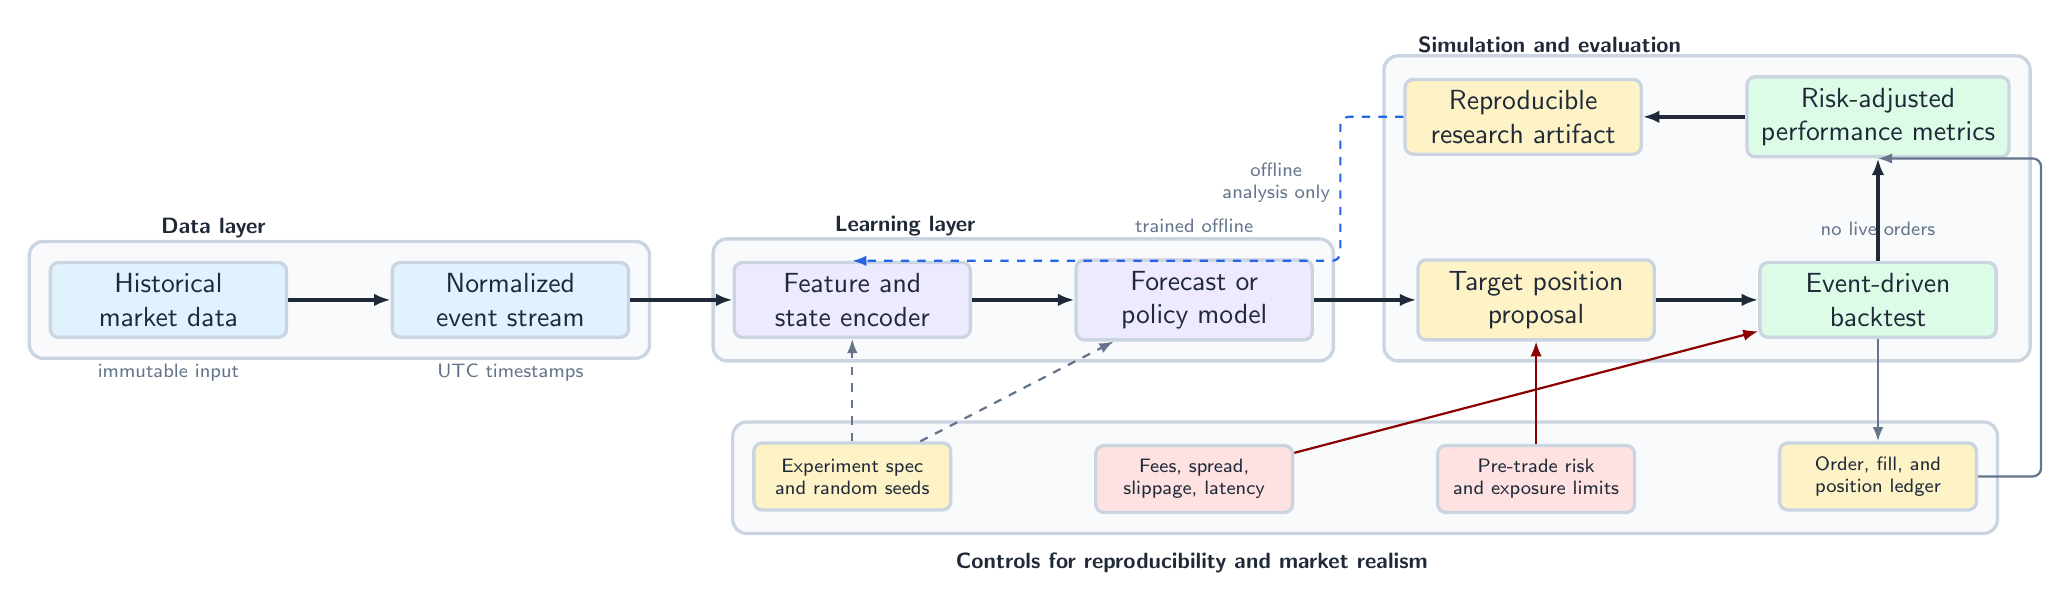
\begin{tikzpicture}[
  font=\sffamily,
  >=Latex,
  node distance=8mm and 13mm,
  module/.style={
    draw=line,
    rounded corners=3pt,
    very thick,
    fill=white,
    minimum width=30mm,
    minimum height=9.5mm,
    inner xsep=5pt,
    inner ysep=4pt,
    align=center,
    text=ink
  },
  smallmodule/.style={
    module,
    minimum width=25mm,
    minimum height=8.5mm,
    font=\sffamily\scriptsize
  },
  title/.style={
    font=\sffamily\bfseries\footnotesize,
    text=ink,
    align=left
  },
  sublabel/.style={
    font=\sffamily\scriptsize,
    text=muted,
    align=center
  },
  flow/.style={
    -{Latex[length=2.1mm,width=1.6mm]},
    very thick,
    draw=ink,
    rounded corners=3pt
  },
  auxflow/.style={
    -{Latex[length=1.8mm,width=1.35mm]},
    thick,
    draw=muted,
    rounded corners=3pt
  },
  guardflow/.style={
    -{Latex[length=1.9mm,width=1.45mm]},
    thick,
    draw=red!55!black,
    rounded corners=3pt
  },
  dashedflow/.style={
    auxflow,
    dashed
  },
  group/.style={
    draw=line,
    rounded corners=5pt,
    fill=panel,
    very thick,
    inner sep=7pt
  }
]

% Core pipeline
\node[module, fill=data] (raw) {Historical\\market data};
\node[module, fill=data, right=of raw] (curated) {Normalized\\event stream};
\node[module, fill=model, right=of curated] (features) {Feature and\\state encoder};
\node[module, fill=model, right=of features] (policy) {Forecast or\\policy model};
\node[module, fill=artifact, right=of policy] (orders) {Target position\\proposal};
\node[module, fill=eval, right=of orders] (sim) {Event-driven\\backtest};

% Governance and realism row
\node[smallmodule, fill=risk, below=13mm of policy] (costs) {Fees, spread,\\slippage, latency};
\node[smallmodule, fill=risk, below=13mm of orders] (risk) {Pre-trade risk\\and exposure limits};
\node[smallmodule, fill=artifact, below=13mm of features] (protocol) {Experiment spec\\and random seeds};
\node[smallmodule, fill=artifact, below=13mm of sim] (ledger) {Order, fill, and\\position ledger};

% Evaluation row
\node[module, fill=eval, above=13mm of sim] (metrics) {Risk-adjusted\\performance metrics};
\node[module, fill=artifact, left=of metrics] (report) {Reproducible\\research artifact};

% Background regions
\begin{scope}[on background layer]
  \node[group, fit=(raw)(curated), label={[title, xshift=-16mm, yshift=-1mm]above:Data layer}] {};
  \node[group, fit=(features)(policy), label={[title, xshift=-15mm, yshift=-1mm]above:Learning layer}] {};
  \node[group, fit=(orders)(sim)(metrics)(report), label={[title, xshift=-20mm, yshift=-1mm]above:Simulation and evaluation}] {};
  \node[group, fit=(protocol)(costs)(risk)(ledger), label={[title, xshift=-22mm, yshift=-1mm]below:Controls for reproducibility and market realism}] {};
\end{scope}

% Main data/control flow
\draw[flow] (raw) -- (curated);
\draw[flow] (curated) -- (features);
\draw[flow] (features) -- (policy);
\draw[flow] (policy) -- (orders);
\draw[flow] (orders) -- (sim);
\draw[flow] (sim) -- (metrics);
\draw[flow] (metrics) -- (report);

% Auxiliary dependencies
\draw[dashedflow] (protocol) -- (features);
\draw[dashedflow] (protocol) -- (policy);
\draw[guardflow] (costs) -- (sim);
\draw[guardflow] (risk) -- (orders);
\draw[auxflow] (sim) -- (ledger);
\draw[auxflow] (ledger.east) -- ++(8mm,0) |- (metrics.south);

% Feedback loop for analysis, intentionally not connected to live execution
\draw[dashedflow, draw=accent]
  (report.west) -- ++(-8mm,0) |- node[pos=0.23, left, sublabel] {offline\\analysis only} (features.north);

\node[sublabel, below=2mm of raw] {immutable input};
\node[sublabel, below=2mm of curated] {UTC timestamps};
\node[sublabel, above=2mm of policy] {trained offline};
\node[sublabel, above=2mm of sim] {no live orders};

\end{tikzpicture}
\end{document}
